\حصہ{فوریئر بدل}
ہم کسی بھی کثافت برقی رو کا پیدا کردہ دور میدان حاصل کرنا دیکھ چکے ہیں۔بعض اوقات ہمیں کثافت برقی رو معلوم نہیں ہوتی البتہ کسی مخصوص سطح پر میدان معلوم ہوتا ہے۔اس طرح کے مسئلے کی مثال مستطیل پیپا اینٹینا ہے۔مستطیل مویج کا منہ کھول کر مستطیل پیپا اینٹینا حاصل کیا جاتا ہے۔اس اینٹینا کے منہ پر کسی قسم کی موصل چادر نہیں نسب کی جاتی لہٰذا اس کے کھلے منہ کے کناروں پر برقی رو پائی جاتی ہے جس کی شکل جاننا دشوار ہے۔البتہ پیپے کی منہ پر برقی میدان جاننا نسبتاً آسان کام ہے۔ہم دیکھیں گے کہ ایسی صورت میں دور میدان قریبی میدان کے \اصطلاح{فوریئر بدل}\فرہنگ{فوریئر بدل!جوڑی}\حاشیہب{Fourier transform pair}\فرہنگ{Fourier transform!pair}  سے حاصل ہوتا ہے۔ آئیں پہلے فوریئر بدل کی یاد دوبارہ تازہ کریں۔
 
آپ فوریئر بدل جوڑی سے بخوبی واقف ہوں گے۔کسی بھی تفاعل \عددی{w(x)} جس کا آزاد متغیرہ \عددی{x} ہو کا فوریئر بدل \عددی{W(k_x)}
\begin{align}\label{مساوات_اینٹینا_فوریئر_بدل_الف}
W(k_x)=\int_{-\infty}^{\infty} w(x) e^{j k_x x} \dif x
\end{align}
لکھا\حاشیہد{عموماً مساوات \حوالہ{مساوات_اینٹینا_فوریئر_بدل_الف} میں تکمل کو \عددی{\tfrac{1}{\sqrt{2\pi}}} سے ضرب دے کر لکھا جاتا ہے۔اسی طرح مساوات \حوالہ{مساوات_اینٹینا_فوریئر_بدل_ب} میں بھی \عددی{\tfrac{1}{2\pi}} کی جگہ \عددی{\tfrac{1}{\sqrt{2\pi}}} سے تکمل کو ضرب دیا جاتا ہے۔اس طرح جوڑی کے دونوں مساوات تقریباً یکساں شکل اختیار کر لیتے ہیں۔} جاتا ہے جہاں \عددی{W(k_x)} کا آزاد متغیرہ \عددی{k_x} ہے۔یوں کسی بھی تفاعل کا آزاد متغیرہ تبدیل کرنا ممکن ہے۔اسی طرح  \عددی{W(k_x)} کا فوریئر بدل \عددی{w(x)} 
\begin{align}\label{مساوات_اینٹینا_فوریئر_بدل_ب}
w(x)=\frac{1}{2\pi}\int_{-\infty}^{\infty} W(k_x)e^{-j k_x x} \dif k_x
\end{align}
ہے۔مندرجہ بالا دو مساوات فوریئر بدل جوڑی کہلاتے ہیں۔ مساوات \حوالہ{مساوات_اینٹینا_فوریئر_بدل_الف} کے  دونوں اطراف کا \عددی{k_x} کے ساتھ تفرق
\begin{align}
\frac{\dif W(k_x)}{\dif k_x}=j k_x \int_{-\infty}^{\infty} w(x) e^{j k_x x} \dif x=j k_x W(k_x)
\end{align}
لکھا جا سکتا ہے۔دائیں ہاتھ تفرق لیتے ہوئے دھیان رہے کہ  تکمل کے اندر \عددی{k_x} کا کردار بالکل ایک مستقل کا ہے لہٰذا تفرق کو تکمل کے اندر لے جایا جا سکتا ہے۔اسی طرح مساوات \حوالہ{مساوات_اینٹینا_فوریئر_بدل_ب} کا تفرق \عددی{x} کے ساتھ لینے سے
\begin{align}
\frac{\dif w(x)}{\dif x}=\frac{-j k_x}{2\pi}\int_{-\infty}^{\infty} W(k_x)e^{-j k_x x} \dif k_x=-j k_x w(x)
\end{align}
حاصل ہوتا ہے۔اسی طرح
\begin{align}
\frac{\dif^{\,2} W(k_x)}{\dif k_x^2}&=(j k_x)^2 W(k_x)=-k_x^2 W(k_x)\\
\frac{\dif^{\,2} w(x)}{\dif x^2}&=(-j k_x)^2 w(x)=-k_x^2 w(x)
\end{align}
بھی لکھے جا سکتے ہیں۔

دو آزاد متغیرات پر مبنی تفاعل \عددی{u(x,y)} کا فوریئر بدل
\begin{align}\label{مساوات_اینٹینا_فوریئر_بدل_پ}
U(k_x,k_y)=\int_{-\infty}^{\infty} \int_{-\infty}^{\infty} u(x,y)e^{j k_x x+ j k_y y} \dif x \dif y
\end{align}
لکھا جاتا ہے۔اس کا واپسی فوریئر بدل
\begin{align}\label{مساوات_اینٹینا_فوریئر_بدل_ت}
u(x,y)=\frac{1}{4\pi^2}\int_{-\infty}^{\infty} \int_{-\infty}^{\infty} U(k_x,k_y)e^{-j k_x x- j k_y y} \dif k_x \dif k_y
\end{align}
ہو گا۔مساوات \حوالہ{مساوات_اینٹینا_فوریئر_بدل_پ} کے تفرق لے کر 
\begin{gather}
\begin{aligned}\label{مساوات_اینٹینا_فوریئر_بدل_ٹ}
\frac{\partial U}{\partial k_x}&=j x U\\
\frac{\partial U}{\partial k_y}&=j y U\\
\frac{\partial^2 U}{\partial k_x^2}&= -x^2 U\\
\frac{\partial^2 U}{\partial k_x \partial k_y}&=-x y U
\end{aligned}
\end{gather}
اور مساوات \حوالہ{مساوات_اینٹینا_فوریئر_بدل_ت} کے تفرق سے
\begin{gather}
\begin{aligned}\label{مساوات_اینٹینا_فوریئر_بدل_ث}
\frac{\partial u}{\partial x}&=-j k_x u\\
\frac{\partial u}{\partial y}&=-j k_y u\\
\frac{\partial^2 u}{\partial x^2}&= -k_x^2 u\\
\frac{\partial^2 u}{\partial x \partial y}&=-k_x k_y u
\end{aligned}
\end{gather}

\begin{figure}
\centering
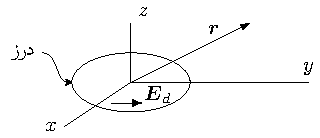
\includegraphics{emtAntennasAndRadiationApertureFourierTransform}
\caption{سطح \عددی{}z=0 پر درز میں برقی میدان \عددی{\kvec{E}_a} کو دور میدان فوریئر بدل ہے۔}
\label{شکل_اینٹینا_درز_فوریئر_بدل}
\end{figure}
فوریئر بدل کی یاد تازہ کرنے کے بعد اصل موضوع پر واپس آتے ہیں۔شکل \حوالہ{شکل_اینٹینا_درز_فوریئر_بدل} میں \عددی{z=0} سطح پر درز دکھایا گیا ہے جس پر برقی میدان \عددی{\kvec{E}_a} ہے۔یہ میدان \عددی{z<0} خطے میں موجود کثافت برقی رو کی وجہ سے پایا جاتا ہے۔ہمیں اس کثافت برقی رو کی ضرورت نہیں پڑے گی۔درز کا رقبہ \عددی{S_a} ہے۔آئیں درز پر موجود میدان سے خالی خلاء میں کہیں دور پیدا میدان دریافت کریں۔ 

میکس ویل کی مساوات \عددی{\nabla \times \kvec{E}=-\tfrac{\partial \kvec{B}}{\partial t}} کے گردش کو
\begin{align*}
\nabla \times \nabla \times \kvec{E}=\nabla \nabla \cdot \kvec{E}-\nabla^2 \kvec{E}&=-j \omega \mu_0 \nabla \times \kvec{H} \\
&=-j \omega \mu_0 (\kvec{J}+j \omega \epsilon_0 \kvec{E})
\end{align*}
لکھا جا سکتا ہے جہاں دوسری قدم پر \عددی{\nabla \times \kvec{H}=\kvec{J}+\tfrac{\partial \kvec{D}}{\partial t}} پر کیا گیا ہے۔ساتھ ہی ساتھ \عددی{\kvec{B}=\mu_0 \kvec{H}} اور \عددی{\kvec{D}=\epsilon_0 \kvec{E}} کے علاوہ \عددی{\tfrac{\partial \kvec{E}}{\partial t}=j \omega \kvec{E}} اور 
\عددی{\tfrac{\partial \kvec{H}}{\partial t}=j \omega \kvec{H}} کا بھی استعمال کیا گیا ہے۔ شکل \حوالہ{شکل_اینٹینا_درز_فوریئر_بدل} میں درز سے دور خالی خلاء میں نہ کوئی کثافت چارج پائی جاتی ہے اور نہ ہی کثافت برقی رو۔یوں مندرجہ بالا مساوات میں دور مقام پر \عددی{\kvec{J}=0} اور  
\begin{align}\label{مساوات_اینٹینا_فوریئر_الف}
\nabla \cdot \kvec{E}&=0
\end{align}
پر کرتے ہوئے
\begin{align}\label{مساوات_اینٹینا_فوریئر_ب}
\nabla^2 \kvec{E}+k_0^2 \kvec{E}=0
\end{align}
حاصل ہوتا ہے جہاں
\begin{align}
k_0= \omega \sqrt{ \mu_0 \epsilon_0}
\end{align}
لکھا گیا ہے۔مساوات \حوالہ{مساوات_اینٹینا_فوریئر_الف} اور مساوات \حوالہ{مساوات_اینٹینا_فوریئر_ب} کو کارتیسی محدد میں یوں لکھا جائے گا۔
\begin{align}
\frac{\partial E_x(x,y,z)}{\partial x}+\frac{\partial E_y(x,y,z)}{\partial y}+\frac{\partial E_z(x,y,z)}{\partial z}&=0 \label{مساوات_اینٹینا_فوریئر_پ}\\
\left(\frac{\partial^2}{\partial x^2}+\frac{\partial^2}{\partial y^2}+\frac{\partial^2}{\partial z^2} +k_0^2\right) \kvec{E}(x,y,z)&=0\label{مساوات_اینٹینا_فوریئر_ت}
\end{align}
ان دو مساوات کا فوریئر بدل مساوات \حوالہ{مساوات_اینٹینا_فوریئر_بدل_ث} کی مدد سے لکھتے ہیں
\begin{align}
k_x E_x(k_x,k_y,k_z)+k_y E_y(k_x,k_y,k_z)+j \frac{\partial E_z(k_x,k_y,k_z)}{\partial z}&=0\label{مساوات_اینٹینا_فوریئر_ٹ}\\
\left[\frac{\partial^2}{\partial z^2}+(k_0^2-k_x^2-k_y^2)\right] \kvec{E}(k_x,k_y,k_z)&=0\label{مساوات_اینٹینا_فوریئر_ث}
\end{align}
 جہاں \عددی{u(x,y,z)=E(x,y,z)} لیتے ہوئے \عددی{U(k_x,k_y,k_z)=E(k_x,k_y,k_z)} لکھا گیا ہے۔یہاں بہتر ہوتا کہ برقی میدان اور اس کے فوریئر بدل کے لئے میں علیحدہ علیحدہ علامات استعمال کرتا لیکن امید کی جاتی ہے کہ \عددی{E(x,y,z)} کے آزاد متغیرات \عددی{(x,y,z)} سے \عددی{E(x,y,z)} کو اصل تفاعل اور \عددی{E(k_x,k_y,k_z)} کے آزاد متغیرات \عددی{(k_x,k_y,k_z)} سے  \عددی{E(k_x,k_y,k_z)}  کو فوریئر بدل سمجھا جا سکتا ہے۔

مندرجہ بالا مساوات میں
\begin{align}
k_0^2-k_x^2-k_y^2=k_z^2
\end{align}
لکھتے ہوئے
\begin{align}
\frac{\partial^2 \kvec{E}(k_x,k_y,k_z)}{\partial z^2}+k_z^2\kvec{E}(k_x,k_y,k_z)&=0
\end{align}
حاصل ہوتا ہے جس کے حل \عددی{e^{\mp j k_z z}} صورت رکھتے ہیں۔ان میں \عددی{e^{-j k_z z}} کارتیسی نظام میں بڑھتے \عددی{z} جانب حرکت کرتی موج ہے جبکہ \عددی{e^{j k_z z}} گھٹتے  \عددی{z} جانب حرکت کرتی موج ہے۔ہم پہلے جواب کو تسلیم کرتے ہیں لہٰذا مندرجہ بالا مساوات کا حل
\begin{align}\label{مساوات_اینٹینا_فوریئر_ج}
\kvec{E}(k_x,k_y,k_z)=\kvec{f}(k_x,k_y) e^{-j k_z z}
\end{align}
لکھا جا سکتا ہے جہاں \عددی{\kvec{f}(k_x,k_y)} دریافت کرنا باقی ہے۔

مساوات \حوالہ{مساوات_اینٹینا_فوریئر_ج} کو مساوات \حوالہ{مساوات_اینٹینا_فوریئر_ٹ} میں پر کرنے سے
\begin{align}
k_x f_x+k_y f_y+k_z f_z=0
\end{align}
یعنی
\begin{align}\label{مساوات_اینٹینا_فوریئر_چ}
\kvec{k} \cdot \kvec{f}=0
\end{align}
ملتا ہے جہاں \عددی{\kvec{f}=f_x \ax+f_y \ay+f_z \az} اور \عددی{\kvec{k}=k_x \ax+k_y \ay+k_z \az} لکھے گئے ہیں۔

برقی میدان \عددی{\kvec{E}(x,y,z)} حاصل کرنے کی خاطر \عددی{\kvec{E}(k_x,k_y,k_z)} کا فوریئر بدل لیتے ہیں
\begin{align*}
\kvec{E}(x,y,z)&=\frac{1}{4\pi^2} \int_{-\infty}^{\infty} \int_{-\infty}^{\infty} \kvec{E}(k_x,k_y,k_z) e^{-j k_x x -j k_y y} \dif k_x \dif k_y\\
&=\frac{1}{4\pi^2} \int_{-\infty}^{\infty} \int_{-\infty}^{\infty} \kvec{f}(k_x,k_y)e^{-j k_x x -j k_y y-j k_z z} \dif k_x \dif k_y
\end{align*}
 جہاں مساوات \حوالہ{مساوات_اینٹینا_فوریئر_ج} استعمال کیا گیا ہے۔کروی محدد کے رداس کو کارتیسی محدد میں \عددی{\kvec{r}=x \ax+y \ay+z \az} لکھا جا سکتا ہے۔یوں  \عددی{k_x x+k_y y+k_z z=\kvec{k}\cdot\kvec{r}} لکھتے ہوئے مندرجہ بالا مساوات کو
\begin{align}
\kvec{E}(x,y,z)&=\frac{1}{4\pi^2} \int_{-\infty}^{\infty} \int_{-\infty}^{\infty} \kvec{f}(k_x,k_y)e^{\kvec{k} \cdot \kvec{r}} \dif k_x \dif k_y
\end{align}
لکھا جا سکتا ہے۔
